\section{用于长消息的无前缀PRF}\label{sec:6-4}

在上一节中,我们看到,任何一个安全的 PRF 也是一个安全的 MAC。然而,第\ref{chap:4}章中的 PRF 实例只接受短的输入,因而只能为非常短的消息提供完整性。比如,如果将 AES 看作是一个 PRF,我们就能得到一个用于 $128$ 比特消息的 MAC。现在,我们想要为更长的消息构建 MAC。

本章中所有的 MAC 构造都遵循同样的范式:它们从短输入的 PRF 开始(如 AES),产生一个 PRF,继而构造一个能用于更长输入的 MAC。因此,我们在本章的剩余部分的目标如下:
\begin{quote}
\textbf{给定一个针对短消息输入的安全 PRF,构建一个针对长消息输入的安全 PRF。}
\end{quote}
我们将会分三步来解决这个问题:
\begin{itemize}
	\item 首先,在本节中,我们为长输入构建\emph{无前缀安全的 PRF}。更确切地说,给定一个在单分组(比如 $128$ 比特)上运行的安全 PRF,我们想要构建一个无前缀的安全 PRF。回顾一下,无前缀安全 PRF(定义 \ref{def:4-5})只在有限的意义上是安全的:我们只要求\emph{无前缀对手}无法区分 PRF 和随机函数。一个无前缀 PRF 对手发出的查询是非空的分组序列,且其中的任何一个查询都不是其他查询的真前缀。
	\item 其次,在接下来的几节中,我们将展示如何把用于长输入的无前缀安全 PRF 转换成用于长输入的完全安全 PRF。因此,在这几节结束时,我们将得到几个这样的安全 PRF,并由此构造出能够用于长消息的安全的 MAC。
	\item 第三,在 \ref{sec:6-8} 节中,我们将展示,如何将一个作用于由分组序列构成的消息的 PRF 转换为一个作用于比特序列的 PRF。
\end{itemize}

\begin{snote}[无前缀的 PRF。]
我们从两个经典的无前缀安全 PRF 构造开始。图 \ref{fig:6-3-a} 展示了 \textbf{CBC} 构造,图 \ref{fig:6-3-b} 展示了\textbf{级联}构造。我们表明,当底层函数 $F$ 是一个安全的 PRF 时,CBC 构造和级联构造都是无前缀安全的 PRF。
\end{snote}

\begin{figure}
  \centering
  \subfigure[CBC构造$F_\mathrm{CBC}(k,m)$]{
  	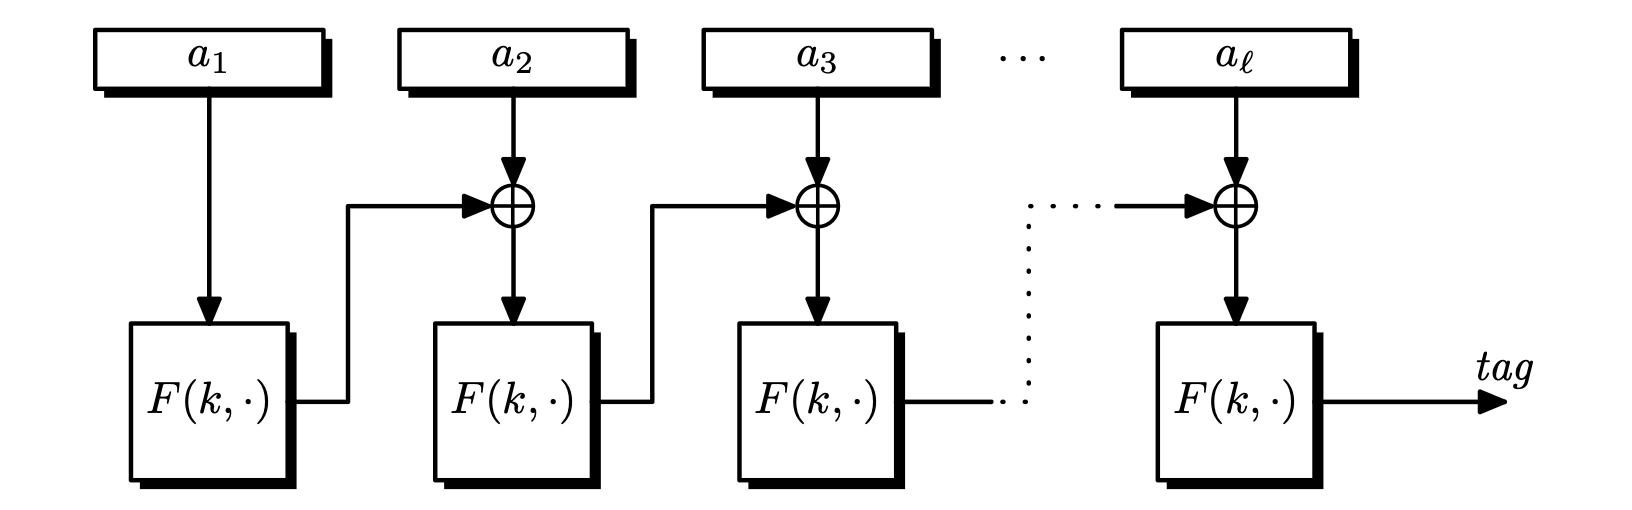
\includegraphics[width=0.8\linewidth]{figures/chapter6/fig3-a.png}
  	\label{fig:6-3-a}
  }
  
  \subfigure[级联构造$F^*(k,m)$]{
  	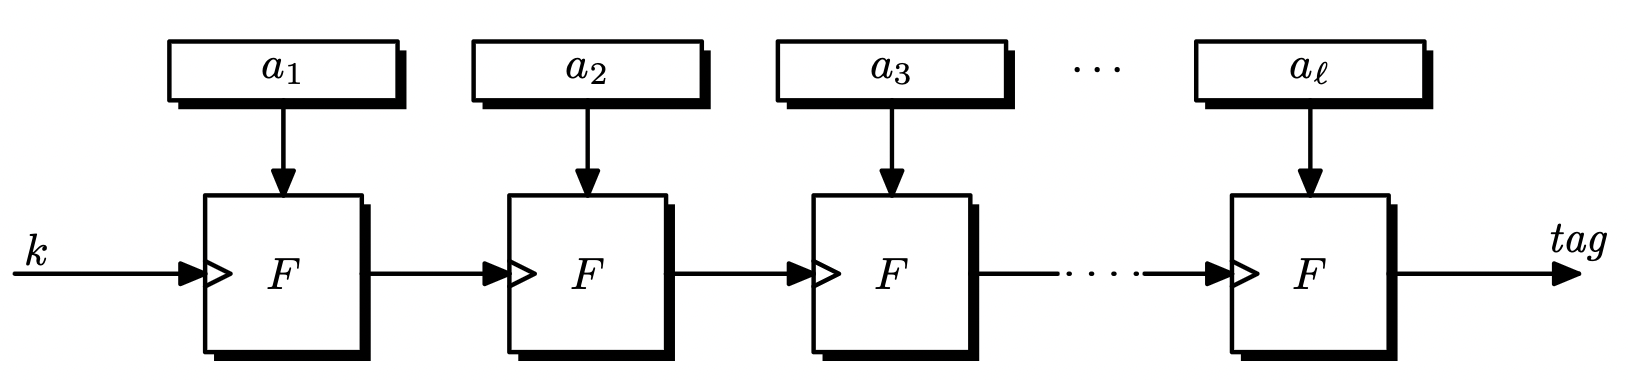
\includegraphics[width=0.8\linewidth]{figures/chapter6/fig3-b.png}
  	\label{fig:6-3-b}
  }
  \caption{两种无前缀安全的 PRF}
\end{figure}

\subsection{CBC无前缀安全PRF}

令 $F$ 是一个 PRF,它将 $n$ 比特的输入映射为 $n$ 比特的输出。$F$ 定义在 $(\mathcal{K},\mathcal{X},\mathcal{X})$ 上,其中 $\mathcal{X}=\{0,1\}^n$。对于任意多项式边界的值 $\ell$,我们构造一个新的 PRF $F_\mathrm{CBC}$,它能够将 $\mathcal{X}^{\leq\ell}$ 上的消息映射为 $\mathcal{X}$ 上的输出。图 \ref{fig:6-3-a} 中描述的函数 $F_\mathrm{CBC}$ 的工作原理如下:

\vspace*{5pt}

\hspace*{5pt} 输入:$k\in\mathcal{K}$ 和 $m=(a_1,\dots,a_v)\in\mathcal{X}^{\leq\ell}$,其中 $v\in\{0,\dots,\ell\}$\\
\hspace*{26pt} 输出:$\mathcal{X}$ 中的一个标签

\vspace*{5pt}

\hspace*{5pt} 令 $t\leftarrow0^n$\\
\hspace*{26pt} 对于 $i=1,\dots,v$:\\
\hspace*{50pt} 计算 $t\leftarrow F(k,\;a_i\oplus t)$\\
\hspace*{26pt} 输出 $t$

\vspace*{5pt}

\noindent
$F_{\rm CBC}$ 与图 \ref{fig:5-4}	中介绍的 CBC 模式加密类似,但是有两个重要的区别。首先,$F_\mathrm{CBC}$ 在 CBC 链中不会输出任何中间值。其次,$F_\mathrm{CBC}$ 使用一个固定的 IV,即 $0^n$,而 CBC 加密对每条消息中都使用一个随机的 IV。

下面的定理表明,$F_\mathrm{CBC}$ 是一种定义在 $(\mathcal{K},\mathcal{X}^{\leq l},\mathcal{X})$ 上的无前缀安全 PRF。

\begin{theorem}\label{theo:6-3}
令 $F$ 是一个定义在 $(\mathcal{K},\mathcal{X},\mathcal{X})$ 上的安全 PRF,其中 $\mathcal{X}=\{0,1\}^n$,$|\mathcal{X}|=2^n$ 是超多项式的。那么,对于任意多项式边界的值 $\ell$,$F_\mathrm{CBC}$ 都是一个定义在 $(\mathcal{K},\mathcal{X}^{\leq\ell},\mathcal{X})$ 上的无前缀安全 PRF。
\begin{quote}
特别地,对于任意如攻击游戏 \ref{game:4-2} 中那样攻击 $F_{\rm CBC}$ 的无前缀 PRF 对手 $\mathcal{A}$,如果它最多能够向其挑战者发起 $Q$ 次查询,则必然存在一个像攻击游戏 \ref{game:4-2} 中那样攻击 $F$ 的 PRF 对手 $\mathcal{B}$,其中 $\mathcal{B}$ 是一个围绕 $\mathcal{A}$ 的基本包装器,满足:
\end{quote}
\begin{equation}\label{eq:6-7}
{\rm PRF^{pf}\mathsf{adv}}[\mathcal{A},F_{\rm CBC}]\leq{\rm PRF\mathsf{adv}}[\mathcal{B},F]+\frac{(Q\ell)^2}{2|\mathcal{X}|}
\end{equation}
\end{theorem}

\noindent
练习 6.6 提出了一种针对定长 $F_\mathrm{CBC}$ 的攻击,并证明其安全性随 $Q$ 的增长而呈二次递减,这表明式 \ref{eq:6-7} 中的 $Q^2$ 项是必要的。一个更困难的安全性证明表明,安全性只随 $\ell$ 的增长线性递减(见第 \ref{sec:6-13} 节)。特别地,式 \ref{eq:6-7} 中的误差项可以被简化为一个以 $O(Q^2\ell/|\mathcal{X}|)$ 为主成分的表达式。

\begin{proof}[证明思路]
我们用一棵有根的树来表示对手的查询,树中的边以消息分组(即 $\mathcal{X}$ 中的元素)为标签。记 $m=(a_1,\dots,a_v)\in\mathcal{X}^{v}$,其中 $1\leq v\leq\ell$,则对 $F(k,m)$ 的一次查询就定义了一条树中的路径,该路径从根开始,如下所示:
\begin{equation}\label{eq:6-8}
root\overset{a_1}\longrightarrow p_1\overset{a_2}\longrightarrow p2 \overset{a_3}\longrightarrow\cdots \overset{a_v}\longrightarrow p_v
\end{equation}
因此,两条消息 $m$ 和 $m'$ 就对应着树中的两条从根开始的路径;这两条路径可能共享一个共同的初始子路径,该子路径就对应着 $m$ 和 $m'$ 的最长公共前缀。

对于这颗树上的每个节点 $p$,我们都将其与一个值 $\gamma_p\in\mathcal{X}$ 关联,该值代表 CBC 链中的计算结果。更确切地说,我们定义 $\gamma_{\rm root}:=0^n$,并且,对于任何非根节点 $q$ 及其父节点 $p$,如果树中的对应路径是 $p\overset{a}\rightarrow q$,那么 $\gamma_q:=F(k,\gamma_p\oplus a)$。有了这些约定,我们可以看到,如果一条消息 $m$ 所对应的路径如式 \ref{eq:6-8} 所示,则有 $\gamma_{p_v}=F_\mathrm{CBC}(k,m)$。

证明的关键是论证:如果 $F$ 表现得像一个随机函数,那么对于树中任意的一对不同的边,比如 $p\overset{a}\rightarrow q$ 和 $p'\overset{a'}\rightarrow q'$,$\gamma_p\oplus a\neq\gamma_{p'}\oplus a'$ 成立的概率都是压倒性的。为了证明不存在这种类型的碰撞,无前缀的限制至关重要,因为它能够保证对手永远不会看到 $\gamma_p$ 和 $\gamma_{p'}$,因此 $a$ 和 $a'$ 与这些值无关。一旦我们确定了不存在这种类型的碰撞,就会发现所有和非根节点相关的值都是随机和独立的,这一点尤其适用于与叶子结点相关的值,它们代表对手所看到的 $F_{\rm CBC}$ 的输出。因此,对手无法将 $F_{\rm CBC}$ 和真随机函数区分开来。
\end{proof}

\begin{proof}
为了让上面的叙述更加严谨,我们让 $\mathcal{A}$ 在四个游戏中与四个密切相关的挑战者进行交互。对于 $j=0,\dots,3$,我们令 $W_j$ 为 $\mathcal{A}$ 在游戏 $j$ 结束后输出 $1$ 的事件。

\vspace{5pt}

\textbf{游戏 $\mathbf{0}$}。
游戏 $0$ 就是攻击游戏 \ref{game:4-2} 的实验 $0$。

\vspace{5pt}

\textbf{游戏 $\mathbf{1}$}。
接下来,和之前一样,我们打出 ``PRF牌",用一个 ${\rm Funs}[\mathcal{X},\mathcal{X}]$ 中的真随机函数 $f$ 代替 $F(k,\cdot)$。显然,对于一个有效对手 $\mathcal{B}$,我们有:
\begin{equation}\label{eq:6-9}
\big\lvert
\Pr[W_1]-\Pr[W_0]
\big\rvert
={\rm PRF}\mathsf{adv}[\mathcal{B},F]
\end{equation}

\textbf{游戏 $\mathbf{2}$}。
接下来,我们做一个纯粹的概念上的改变,用``忠实的侏儒" 来实现随机函数 $f$(如 \ref{subsec:4-4-2} 小节中那样)。然而,我们以一种特殊的方式来进行实现,即使用上面介绍的``查询树"。

为此,我们首先令 $B:=Q\ell$,它代表 $f$ 被计算的次数的上界。我们的挑战者首先准备一系列的随机数:
\[
\beta_i\overset{\rm R}\leftarrow\mathcal{X}\quad
(i=1,\dots,B)
\]
这些随机数将会是我们的挑战者在游戏中所使用的仅有的几个随机值。

随着对手的查询,我们的挑战者将动态地建立起它的查询树。最初,查询树只有一个树根。每当对手进行查询时,挑战者就会在现有的查询树中加入新的路径;在某些时候,这个路径可能会延伸到现有的查询树之外,那么挑战者就会向树中添加必要的节点和边,以使查询树能够容纳新的查询路径。

我们的挑战者还必须计算与每个节点相关的 $\gamma_p$ 值。在最开始时,它只有 $\gamma_{\rm root}=0^n$。当在树中添加一条新边 $p\overset{a}\rightarrow q$ 时,如果这是被添加的第 $i$ 条边(对于 $i=1,\dots,B$),我们的挑战者会进行以下操作:

\vspace{8pt}

\hspace*{5pt} 令 $\gamma_q\leftarrow\beta_i$\\
\hspace*{1pt} ($*$)
\hspace*{4.5pt} 如果存在另一条边 $p'\overset{a'}\rightarrow q'$ 使得 $\gamma_{p'}\oplus a'=\gamma_p\oplus a$,则令 $\gamma_q\leftarrow\gamma_{q'}$

\vspace{8pt}

\noindent
我们的想法是,在我们准备的序列 $\beta_1,\dots,\beta_B$ 使用下一个还未使用的值作为 $\gamma_q$ 的``默认"值。标有 ($*$) 的那行进行了必要的一致性检查,这确保了我们的侏儒确实是忠实的。

由于这种修改纯粹只是概念上的,我们有:
\begin{equation}\label{eq:6-10}
\Pr[W_2]=\Pr[W_1]
\end{equation}

\textbf{游戏 $\mathbf{3}$}。
接下来,我们通过删除游戏 $2$ 中标有 ($*$) 的那行,使得我们的侏儒变得健忘。

为了分析这一变化的影响,令 $Z$ 为\emph{在游戏 3 中},存在不同的两条边 $p\overset{a}\rightarrow q$ 和 $p'\overset{a'}\rightarrow q'$ 使得 $\gamma_{p'}\oplus a'=\gamma_p\oplus a$ 成立的事件。

现在,游戏 $2$ 和游戏 $3$ 中唯一随机选择的值就是对手的随机选择,即$Coins$,以及一系列的 $\beta_1,\dots,\beta_B$。注意到,对于任意固定的 $Coins,\beta_1,\dots,\beta_B$ 的随机选择,如果 $Z$ 没有发生,那么实际上游戏 $2$ 和游戏 $3$ 的进程就是完全相同的。因此,我们可以利用差分引理(定理 \ref{theo:4-7}),得到:
\begin{equation}\label{eq:6-11}
\big\lvert\Pr[W_3]-\Pr[W_2]\big\rvert\leq\Pr[Z]
\end{equation}

接下来,我们约束 $\Pr[Z]$。考察两条不同的边 $p\overset{a}\rightarrow q$ 和 $p'\overset{a'}\rightarrow q'$。我们想要约束 $\gamma_{p'}\oplus a'=\gamma_p\oplus a$ 成立的概率。该等式与:
\begin{equation}\label{eq:6-12}
\gamma_{p'}\oplus\gamma_p =a'\oplus a
\end{equation}
等价。有两种情况需要考虑:

\emph{情况1:}$p=p'$。由于两条边是不同的,我们必有 $a'\neq a$,因此式 \ref{eq:6-12} 成立的概率为 $0$。

\emph{情况2:}$p\neq p'$。对手查询是无前缀的,这一要求意味着在游戏 $3$ 中,对手永远不会看到或了解到关于 $\gamma_p$ 和 $\gamma_{p'}$ 的任何信息。$p$ 和 $p'$ 中的一个可能是根节点,但不可能两个都是。由此可见,$\gamma_{p'}\oplus\gamma_p$ 的值均匀分布在 $\mathcal{X}$ 上,且与 $a\oplus a'$ 无关。因此,式 \ref{eq:6-12} 成立的概率为 ${1}/{|\mathcal{X}|}$。

根据联合约束,可以得到:
\begin{equation}\label{eq:6-13}
\Pr[Z]\leq\frac{B^2}{2|\mathcal{X}|}
\end{equation}

将式 \ref{eq:6-9},\ref{eq:6-10},\ref{eq:6-11} 和\ref{eq:6-13} 相结合,我们得到:
\begin{equation}\label{eq:6-14}
{\rm PRF^{pf}}\mathsf{adv}[\mathcal{A},F_{\rm CBC}]=
\big\lvert\Pr[W_3]-\Pr[W_0]\big\rvert\leq{\rm PRF}\mathsf{adv}[\mathcal{B},F]+\frac{B^2}{2|\mathcal{X}|}
\end{equation}
此外,游戏 $3$ 完全对应于攻击游戏 \ref{game:4-2} 的实验 $1$,因此,该定理得证。
\end{proof}

\subsection{级联无前缀安全PRF}\label{subsec:6-4-2}

令 $F$ 是一个 PRF,它接受 $\mathcal{K}$ 中的密钥并输出 $\mathcal{K}$ 中的元素。我们称 $F$ 定义在 $(\mathcal{K},\mathcal{X},\mathcal{K})$ 上。对于任意多项式边界的值 $\ell$,我们建立一个新的 PRF $F^*$,称为 \textbf{$F$ 的级联 (cascade of $F$)},它将 $\mathcal{X}^{\leq\ell}$ 中的消息映射为 $\mathcal{K}$ 上的输出,如图 \ref{fig:6-3-b} 所示,该构造的原理如下:

\vspace*{5pt}

\hspace*{5pt} 输入:$k\in\mathcal{K}$ 和 $m=(a_1,\dots,a_v)\in\mathcal{X}^{\leq\ell}$,其中 $v\in\{0,\dots,\ell\}$\\
\hspace*{26pt} 输出:$\mathcal{K}$ 中的一个标签

\vspace*{5pt}

\hspace*{5pt} 令 $t\leftarrow k$\\
\hspace*{26pt} 对于 $i=1,\dots,v$:\\
\hspace*{50pt} 计算 $t\leftarrow F(t,\;a_i)$\\
\hspace*{26pt} 输出 $t$

\vspace*{5pt}

\noindent
下面的定理将表明,$F^*$ 是一个无前缀安全的 PRF。

\begin{theorem}\label{theo:6-4}
令 $F$ 是一个定义在 $(\mathcal{K},\mathcal{X},\mathcal{K})$ 上的安全的 PRF。那么,对于任意多项式边界的值 $\ell$,$F$ 的级联 $F^*$ 是一个定义在 $(\mathcal{K},\mathcal{X}^{\leq\ell},\mathcal{K})$ 上的无前缀安全的 PRF。
\begin{quote}
特别地,对于任意如攻击游戏 \ref{game:4-2} 中那样攻击 $F^*$ 的无前缀 PRF 对手 $\mathcal{A}$,假设它最多能够向其挑战者发起 $Q$ 次查询,则必然存在一个像攻击游戏 \ref{game:4-2} 中那样攻击 $F$ 的 PRF 对手 $\mathcal{B}$,其中 $\mathcal{B}$ 是一个围绕 $\mathcal{A}$ 的基本包装器,满足:
\end{quote}
\begin{equation}\label{eq:6-15}
{\rm PRF^{pf}\mathsf{adv}}[\mathcal{A},F^*]\leq Q\ell\cdot{\rm PRF\mathsf{adv}}[\mathcal{B},F]
\end{equation}
\end{theorem}

练习 6.6 提出了一种针对定长 $F^*$ 的攻击,并证明其安全性随 $Q$ 的增长而四次方递减。这令人不安,因为它似乎与式 \ref{eq:6-15} 中对 $Q$ 的线性依赖相矛盾。然而,请读者放心,这里其实并没有矛盾。练习 6.6 中的对手使用 $\ell=3$,当 $Q$ 大约为 $\sqrt{|\mathcal{K}|}$ 时,其优势约为 $1/2$。将 $\mathcal{A}$ 接入定理 \ref{theo:6-4} 的证明中,我们就能够得到一个 PRF 对手 $\mathcal{B}$,它在攻击 PRF $F$ 时大约进行 $Q$ 次查询,获得的优势大约是 $1/Q$。注意到,当 $Q$ 接近 $\sqrt{|\mathcal{K}|}$ 时,我们有 $1/Q\approx|\mathcal{K}|$ 这样的近似关系。这样的对手 $\mathcal{B}$ 并不令人惊讶:它本质上就是练习 4.27 中的通用 PRF 攻击者。因此,式 \ref{eq:6-15} 与练习 6.6 中的攻击本质上是一致的。另一种视角是,式 \ref{eq:6-15} 中已经出现了对 $Q$ 的二次依赖,因为有一个隐藏的 $Q$ 的因子被包含在了 ${\rm PRF\mathsf{adv}}[\mathcal{B},F]$ 这个量中。

\vspace{5pt}

证明定理 \ref{theo:6-4} 与证明 \ref{sec:4-6} 节中的变长树构造是一个无前缀安全的 PRF(定理 \ref{theo:4-11})是相似的。我们下面简单介绍一下如何扩展定理 \ref{theo:4-11} 的证明来证明定理 \ref{theo:6-4}。

\begin{snote}[与树构造的关系。]
级联构造是 \ref{sec:4-6} 节中介绍的变长树构造的一个推广。回顾一下,树构造使用一个安全的 PRG 建立一个安全的 PRF,该 PRG 将一个种子映射到一对种子。不难发现,当 $F$ 是定义在 $(\mathcal{K},\{0,1\},\mathcal{K})$ 上的 PRF 时,定理 \ref{theo:6-4} 就是定理 \ref{theo:4-11} 的直接推论:我们只要定义 PRG $G$ 为 $G(k):=(F(k,0),F(k,1))\in\mathcal{K}^2$,并且观察到用于 $F$ 的级联构造与用于 $G$ 的变长树构造本质上是相同的。

定理 \ref{theo:4-11} 的证明很容易推广到对任何 PRF 证明定理 \ref{theo:6-4}。比如说,假设 $F$ 定义在 $(\mathcal{K},\{0,1,2\},\mathcal{K})$ 上,那么它就对应于一个 PRF $G$,它将 $k\in\mathcal{K}$ 映射为 $G(k):=(F(k,0),F(k,1),F(k,2))\in\mathcal{K}^3$。如果我们将用于 $F$ 的级联构造看作是一颗三叉树而不是二叉树,那么甚至不需要修改太多,就可以套用定理 \ref{theo:4-11} 的证明。

但为什么要在宽度为 $3$ 的情况下停止呢?我们可以按我们的期望任意设定树的宽度。基于一个定义在 $(\mathcal{K},\mathcal{X},\mathcal{K})$ 上的PRF $F$ 的级联构造就对应于一棵宽度为 $|\mathcal{X}|$ 的树。同样地,定理 \ref{theo:4-11} 的证明也没有发生本质的变化。我们把细节留给感兴趣的读者作为练习(可以参考练习 4.26)。
\end{snote}

\begin{snote}[CBC 和级联 PRF 的对比。]
请注意,CBC 对 $F$ 的所有应用都使用同一个固定的密钥 $k$,而级联构造在每一轮中都使用不同的密钥。由于分组密码通常会使用相同的密钥来加密许多分组,因此级联构造中的密钥更新有可能导致比 CBC 更差的性能。因此,当使用像 AES 这样的现成的分组密码时,CBC 是更加自然的选择。

级联构造的一个优点是,式 \ref{eq:6-15} 中的上界中没有误差项。因此,即使底层 PRF 所依赖的领域 $\mathcal{X}$ 相对较小,级联构造仍然是安全的。相对地,CBC 只有在 $\mathcal{X}$ 大的时候才是安全的。因此,级联构造可以用来将 PRG 转换成大输入的 PRF,而 CBC 不能。
\end{snote}

\subsection{CBC 和级联 PRF 都是不安全的 MAC}

我们表明,从 CBC 和级联构造派生出来的 MAC 都是不安全的。这意味着 CBC 和级联构造都不是安全的 PRF。而我们在之前的章节中所展示的只是,CBC 和级联构造是\emph{无前缀}安全的 PRF。

\begin{snote}[对级联构造的扩展攻击。]
对于 $\mathcal{X}^{\leq\ell}$ 中的某条消息 $m$,给定 $F^*(k,m)$,对于任何的 $m'\in\mathcal{X}^*$,即使不知道 $k$,任何人也都能计算:
\begin{equation}\label{eq:6-16}
t':=F^*(k,\;m\,\Vert\,m')
\end{equation}
一旦 $F^*(k,m)$ 已知,任何人都可以用消息 $m'$ 的分组继续评估链,并最终得到 $t'$。我们把这称为级联构造的\textbf{扩展属性 (extension property)}。

扩展属性意味着,由 $F^*$ 派生而来的 MAC 是非常不安全的。伪造者可以首先请求消息 $m$ 的 MAC,然后对于任意的 $m'$,伪造者都可以推导出 $m\,\Vert\,m'$ 的 MAC。因此,根据定理 \ref{theo:6-2},$F^*$ 不是一个安全的 PRF。
\end{snote}

\begin{snote}[一种针对 CBC 的攻击。]
我们下面描述一种针对由 CBC 派生出的 MAC 的 MAC 伪造器。该伪造器的工作原理如下:
\begin{enumerate}
	\item 挑选一个任意的 $a_1\overset{\rm R}\leftarrow\mathcal{X}$;
	\item 请求单分组消息 $(a_1)$ 的标记 $t$;
	\item 定义 $a_2:=a_1\oplus t$,并输出 $t$ 作为两分组消息 $(a_1,a_2)\in\mathcal{X}$ 的 MAC 伪造。
\end{enumerate}
注意到 $t=F(k,a_1)$,$a_1=F(k,a_1)\oplus a_2$。根据 CBC 的定义,我们有:
\[
F_{\rm CBC}(k,(a_1,a_2))=F(k,F(k,a_1)\oplus a_2)=F(k,a_1)=t
\]
因此,$((a_1,a_2),t)$  是一个针对由 CBC 派生的 MAC 的存在性伪造。所以 $F_{\rm CBC}$ 无法成为一个安全的 PRF。请注意,对级联构造 MAC 的攻击远比对 CBC MAC 的攻击更具破坏性。但无论如何,这些攻击都表明,CBC 和级联构造都不应该被直接当作 MAC 使用。
\end{snote}